% ------------------------------------------------------------------------
% ------------------------------------------------------------------------
% Modelo UFSC para Trabalhos Academicos (tese de doutorado, dissertação de
% mestrado) utilizando a classe abntex2
%
% Autor: Alisson Lopes Furlani
% 	Modificações:
%	- 27/08/2019: Alisson L. Furlani, add pacote 'glossaries' para listas
% - 30/10/2019: Alisson L. Furlani, adjusted some spacing errors and changed math fonts
% - 17/01/2019: Alisson L. Furlani, updated certification page
% - 03/03/2020: Luiz F. P. Droubi, change file to be used as a template with R.
% ------------------------------------------------------------------------
% ------------------------------------------------------------------------

\documentclass[
	% -- opções da classe memoir --
	12pt,				% tamanho da fonte
	%openright,			% capítulos começam em pág ímpar (insere página vazia caso preciso)
	oneside,			% para impressão no anverso. Oposto a twoside
	a4paper,			% tamanho do papel.
	% -- opções da classe abntex2 --
	chapter=TITLE,		% títulos de capítulos convertidos em letras maiúsculas
	section=TITLE,		% títulos de seções convertidos em letras maiúsculas
	%subsection=TITLE,	% títulos de subseções convertidos em letras maiúsculas
	%subsubsection=TITLE,% títulos de subsubseções convertidos em letras maiúsculas
	% -- opções do pacote babel --
	english,			% idioma adicional para hifenização
	%french,				% idioma adicional para hifenização
	%spanish,			% idioma adicional para hifenização
	brazil				% o último idioma é o principal do documento
	]{abntex2}

\usepackage{setup/ufrnthesisA4-alf}

\addbibresource{bib/thesis.bib}
\addbibresource{bib/discussion.bib}
\addbibresource{bib/pkgs.bib}

\usepackage[table]{xcolor}
\let\newfloat\undefined
\usepackage{floatrow}
\floatsetup[table]{capposition=top}
\floatsetup[figure]{capposition=top}

\newcommand{\pkg}[1]{{\normalfont\fontseries{b}\selectfont #1}}
\let\proglang=\textsf
\let\code=\texttt


\newcommand{\bcenter}{\begin{center}}
\newcommand{\ecenter}{\end{center}}

\newcommand{\bapendices}{\begin{apendicesenv}}
\newcommand{\eapendices}{\end{apendicesenv}}

\newcommand{\banexos}{\begin{anexosenv}}
\newcommand{\eanexos}{\end{anexosenv}}

% ---
% Filtering and Mapping Bibliographies
% ---
\DeclareSourcemap{
	\maps[datatype=bibtex]{
		% remove fields that are always useless
		\map{
			\step[fieldset=abstract, null]
			\step[fieldset=pagetotal, null]
		}
		% remove URLs for types that are primarily printed
%		\map{
%			\pernottype{software}
%			\pernottype{online}
%			\pernottype{report}
%			\pernottype{techreport}
%			\pernottype{standard}
%			\pernottype{manual}
%			\pernottype{misc}
%			\step[fieldset=url, null]
%			\step[fieldset=urldate, null]
%		}
		\map{
			\pertype{inproceedings}
			% remove mostly redundant conference information
			\step[fieldset=venue, null]
			\step[fieldset=eventdate, null]
			\step[fieldset=eventtitle, null]
			% do not show ISBN for proceedings
			\step[fieldset=isbn, null]
			% Citavi bug
			\step[fieldset=volume, null]
		}
	}
}
% ---

% ---
% Informações de dados para CAPA e FOLHA DE ROSTO
% ---
% FIXME Substituir 'Nome completo do autor' pelo seu nome.
\autor{JOÃO VITOR FERREIRA CAVALCANTE}
% FIXME Substituir 'Título do trabalho' pelo título da trabalho.
\titulo{O Ecossistema Computacional da Metagenômica}
% FIXME Substituir 'Subtítulo (se houver)' pelo subtítulo da trabalho.
% Caso não tenha substítulo, comente a linha a seguir.
  \subtitulo{Fluxos de Trabalho e Reprodutibilidade}
% FIXME Substituir 'XXXXXX' pelo nome do seu
% orientador.
\orientador{Rodrigo Juliani Siqueira Dalmolin}
% FIXME Se for orientado por uma mulher, comente a linha acima e descomente a linha a seguir.
% \orientador[Orientadora]{Nome da orientadora, Dra.}
% FIXME Substituir 'XXXXXX' pelo nome do seu
% coorientador. Caso não tenha coorientador, comente a linha a seguir.
% FIXME Se for coorientado por uma mulher, comente a linha acima e descomente a linha a seguir.
% \coorientador[Coorientadora]{XXXXXX, Dra.}
% FIXME Substituir '[ano]' pelo ano (ano) em que seu trabalho foi defendido.
\ano{2024}
% FIXME Substituir '[dia] de [mês] de [ano]' pela data em que ocorreu sua defesa.
\data{06 de Dezembro de 2024}
% FIXME Substituir 'Local' pela cidade em que ocorreu sua defesa.
\local{NATAL - RN}
\instituicaosigla{UFRN}
\instituicao{Universidade Federal do Rio Grande do Norte}
% FIXME Substituir 'Dissertação/Tese' pelo tipo de trabalho (Tese, Dissertação).
\tipotrabalho{Defesa de Mestrado}
% FIXME Substituir '[mestre/doutor] em XXXXXX' pela grau adequado.
\formacao{Mestre em Bioinformática}
% FIXME Substituir '[mestrado/doutorado]' pelo nivel adequado.
\nivel{mestrado}
% FIXME Substituir 'Programa de Pós-Graduação em XXXXXX' pela curso adequado.
\programa{Programa de Pós-Graduação em Bioinformática}
% FIXME Substituir 'Campus XXXXXX ou Centro de XXXXXX' pelo campus ou centro adequado.
\centro{Instituto Metrópole Digital}
\preambulo
{%
\imprimirtipotrabalho~apresentada~ao~\imprimirprograma~da~\imprimirinstituicao.
}
% ---

% ---
% Configurações de aparência do PDF final
% ---
% alterando o aspecto da cor azul
\definecolor{blue}{RGB}{41,5,195}
% informações do PDF
\makeatletter
\hypersetup{
     	%pagebackref=true,
		pdftitle={\@title},
		pdfauthor={\@author},
    	pdfsubject={\imprimirpreambulo},
	    pdfcreator={LaTeX with abnTeX2},
		pdfkeywords={ufsc, latex, abntex2},
		colorlinks=true,       		% false: boxed links; true: colored links
    	linkcolor=black,%blue,          	% color of internal links
    	citecolor=black,%blue,        		% color of links to bibliography
    	filecolor=black,%magenta,      		% color of file links
		urlcolor=black,%blue,
		bookmarksdepth=4
}
\makeatother
% ---

% ---
% compila a lista de abreviaturas e siglas e a lista de símbolos
% ---

% Declaração das siglas
\siglalista{MS}{metagenômica \textit{shotgun}}
\siglalista{16S}{sequenciamento da subunidade ribossomal 16S de genomas bacterianos}
\siglalista{TDM}{transtorno depressivo maior}
\siglalista{DNA}{Ácido Desoxirribonucléico}
\siglalista{OTU}{unidades taxonômicas operacionais - do inglês \textit{operational taxonomic units}}
\siglalista{ASV}{variantes de sequência amplicon - do inglês \textit{amplicon sequence variant}}


% Declaração dos simbolos
\simbololista{C}{\ensuremath{C}}{Circunferência de um círculo}
\simbololista{pi}{\ensuremath{\pi}}{Número pi}
\simbololista{r}{\ensuremath{r}}{Raio de um círculo}
\simbololista{A}{\ensuremath{A}}{Área de um círculo}


% compila a lista de abreviaturas e siglas e a lista de símbolos
\makenoidxglossaries

% ---

% ---
% compila o indice
% ---
\makeindex
% ---

% ----
% Início do documento
% ----
\begin{document}

% Seleciona o idioma do documento (conforme pacotes do babel)
%\selectlanguage{english}
\selectlanguage{brazil}

% Retira espaço extra obsoleto entre as frases.
\frenchspacing

% Espaçamento 1.5 entre linhas
\OnehalfSpacing

% Corrige justificação
%\sloppy

% ----------------------------------------------------------
% ELEMENTOS PRÉ-TEXTUAIS
% ----------------------------------------------------------
% \pretextual %a macro \pretextual é acionado automaticamente no início de \begin{document}
% ---
% Capa, folha de rosto, ficha bibliografica, errata, folha de apróvação
% Dedicatória, agradecimentos, epígrafe, resumos, listas
% ---
% ---
% Capa
% ---
\imprimircapa
% ---

% ---
% Folha de rosto
% (o * indica que haverá a ficha bibliográfica)
% ---
\imprimirfolhaderosto*
% ---

% ---
% Inserir a ficha bibliografica
% ---
% http://ficha.bu.ufsc.br/
% \begin{fichacatalografica}
% 	\includepdf{Ficha_Catalografica.pdf}
% \end{fichacatalografica}
% ---

% ---
% Inserir folha de aprovação
% ---
\begin{folhadeaprovacao}
	\OnehalfSpacing
	% \centering
	\begin{center}
	\imprimirautor\\%
	\vspace*{10pt}
	\textbf{\imprimirtitulo}%
	\ifnotempty{\imprimirsubtitulo}{:~\imprimirsubtitulo}\\%
	%		\vspace*{31.5pt}%3\baselineskip
	\vspace*{\baselineskip}
	\end{center}
	%\begin{minipage}{\textwidth}
	\imprimirtipotrabalho~apresentada~ao~\imprimirprograma~da~\imprimirinstituicao\\
	%\end{minipage}%
	\bigskip\newline
	\textbf{Área de Concentração}:~Bioinformática\newline%
	\textbf{Linha de Pesquisa}:~Biologia de Sistemas\newline%
	\imprimirorientadorRotulo:~\imprimirorientador\newline%
	\begin{flushright}
	Natal, \imprimirdata.
	\end{flushright}
	\vspace*{\baselineskip}
  %   % Prof. Renan Cipriano Moioli, Dr.\\
  % Universidade Federal do Rio Grande do Norte - UFRN\\
  % \vspace*{\baselineskip}
  %   % Prof. Daniel Carlos Ferreira Lanza, Dr.\\
  % Universidade Federal do Rio Grande do Norte - UFRN\\
  % \vspace*{\baselineskip}
  %   % Prof. Marcel da Câmara Ribeiro-Dantas, Dr.\\
  % Universidade Potiguar - UNP\\
  % \vspace*{\baselineskip}
  % 
	\vspace*{2\baselineskip}
	% \begin{minipage}{\textwidth}
	% 	Certificamos que esta é a \textbf{versão original e final} do trabalho de conclusão que foi julgado adequado para obtenção do título de \imprimirformacao.\\
	% \end{minipage}
	%    \vspace{-0.7cm}
	\centering{\textbf{BANCA EXAMINADORA}}
	\assinatura{\OnehalfSpacing Prof. Dr. \imprimirorientador \\ \footnotesize{\imprimirinstituicao \\ (Presidente)}}
    \assinatura{Prof. Dr. Renan Cipriano Moioli \\ \footnotesize{Universidade Federal do Rio Grande do Norte \\ (Examinador Interno do Programa)}}
    \assinatura{Prof. Dr. Daniel Carlos Ferreira Lanza \\ \footnotesize{Universidade Federal do Rio Grande do Norte \\ (Examinador Interno do Programa)}}
    \assinatura{Prof. Dr. Marcel da Câmara Ribeiro-Dantas \\ \footnotesize{Universidade Potiguar \\ (Examinador Externo à Instituição)}}
  	%	\ifnotempty{\imprimircoorientador}{
	%	\assinatura{\imprimircoorientador \\ \imprimircoorientadorRotulo \\
	%		\imprimirinstituicao~--~\imprimirinstituicaosigla}
	%	}
	% \newpage
	\vspace*{\fill}
	\centering
\end{folhadeaprovacao}
% ---

% ---
% Dedicatória
% ---
\begin{dedicatoria}
	\vspace*{\fill}
	\noindent
	\begin{adjustwidth*}{}{5.5cm}
		\raggedleft
		Para meus pais, que me mostraram que isso era possível.
	\end{adjustwidth*}
\end{dedicatoria}
% ---

% ---
% Agradecimentos
% ---
\begin{agradecimentos}
	Agradeço a meus amigos do BioME, colegas na jornada acadêmica, que me forneceram várias discussões, sobre pesquisa ou não, várias descontrações - a tradição do 4 e mate - e várias (necessárias) distrações, além de muitas e muitas perguntas.\\
Mais que tudo isso, vocês me deram o sentimento de fazer de parte de uma comunidade. Agradeço a todos vocês, mas em especial a Julia, ao Diego, ao Epitácio, ao Gleison, ao Bruno e a Bianca.\\
\strut \\
Agradeço ao Rodrigo, por me dar tanta liberdade para executar meu trabalho, pela confiança constante no meu futuro e no caminho que estou trilhando e pelos conselhos quando este caminho dá algumas voltas caóticas.\\
\strut \\
Agradeço aos amigos do grupo Código Bonito, em especial Tiago, Kléber e Vini. Obrigado por confiar no meu trabalho o suficiente para me recomendar para vagas e eventos, que fizeram uma diferença inestimável na minha trajetória e me proporcionaram com novas experiências, amizades e perspectivas.\\
\strut \\
Agradeço aos amigos feitos nesses vários eventos, alguns já citados aqui, mas em especial Débora, Pedro e Igor.\\
\strut \\
Agradeço às instituições brasileiras que me possibilitaram fazer pesquisa.\\
\strut \\
Agradeço a Beatriz, que sabe que seu impacto é tanto que apenas algumas linhas em um documento sobretudo acadêmico seria insuficiente ou talvez desrespeitoso, e que também sabe que já te agradeço tanto em tudo que faço a ponto de ficar repetitivo.\\
Te amo, estou aqui por causa de ti e para ti.
\end{agradecimentos}
% ---

% ---
% Epígrafe
% ---
\begin{epigrafe}
	\vspace*{\fill}
	\begin{flushright}
		\textit{``Nature uses only the longest threads to weave her patterns, so that each small piece of her fabric reveals the organization of the entire tapestry.''\\
(Richard P. Feynman)}
	\end{flushright}
\end{epigrafe}
% ---

% ---
% RESUMOS
% ---

% resumo em português
\setlength{\absparsep}{18pt} % ajusta o espaçamento dos parágrafos do resumo
\begin{resumo}
	\SingleSpacing
  Os últimos anos têm testemunhado avanços significativos no estudo de comunidades microbianas complexas, impulsionados pela evolução das tecnologias de sequenciamento e pela crescente adoção de métodos de sequenciamento total do genoma (whole genome shotgun) em detrimento dos métodos, antes mais tradicionais, baseados em amplicon. Com essa evolução, essas abordagens foram desenvolvidas com estratégias computacionais associadas para lidar com os dados que geram. No entanto, esses métodos computacionais geralmente não foram acompanhados por estratégias de design cuidadosas que priorizam o suporte a longo prazo, com baixa necessidade de manutenção, alta acessibilidade de dados e automação de ponta a ponta.

  Neste trabalho, nosso objetivo é, primeiramente, elaborar sobre o cenário computacional em metagenômica e como os métodos atuais podem negligenciar princípios fundamentais de desenvolvimento de software, que os orientariam para uma maior reprodutibilidade, tais como isolamento de dependências, alta parametrização, geração automática de relatórios com figuras interativas que facilitam a exploração de dados e, por fim, documentação descritiva e prática. Em seguida, abordamos as limitações atuais no processamento de dados metagenômicos ao implementar um novo pipeline de análise de dados, o EURYALE, baseado em uma metodologia anterior, o MEDUSA, que selecionou suas ferramentas por meio de rigoroso benchmarking. Esse novo pipeline, adaptável a diferentes cenários e construído com boas práticas de desenvolvimento de software como princípios norteadores, visa avançar o processamento de dados metagenômicos como um todo e, adicionalmente, tornar os dados resultantes desses pipelines de análise acessíveis a um público mais amplo.

  \textbf{Palavras-chave}:
    Metagenômica.
    Fluxos de Trabalho.
    Reprodutibilidade.
    Desenvolvimento de Software.
    Nextflow.
  \end{resumo}
% resumo em inglês
\begin{resumo}[Abstract]
	\SingleSpacing
	\begin{otherlanguage*}{english}
		The past few years have seen significant advances in the study of complex microbial communities associated with the evolution of sequencing technologies and increasing adoption of whole genome shotgun sequencing methods over the once more traditional Amplicon-based methods.
Through this evolution, these approaches have been built with associated computational strategies to tackle the data they generate. However,
these computational methods have not been generally accompanied by thoughtful design strategies that prioritise long term support with low maintainability, high data accessibility and end-to-end automation.

In this work, we aim to first elaborate on the computational landscape in metagenomics, and how its methods can disregard fundamental software development principles that guide them towards improved reproducibility, principles such as dependency isolation, high parameterization, automatic report generation, with interactive figures that facilitate data exploration and, finally, descriptive and practical documentation. Following this, we tackle current limitations in metagenomic data processing by implementing a new data analysis pipeline, EURYALE, based on a previous methodology, MEDUSA, that selected its tools through rigorous benchmarking. This new pipeline, adaptable to different scenarios and built with good software development practices as guiding principles, serves to advance metagenomic data processing as a whole, and, additionally, make the data resulting from these analysis pipelines accessible to a wider audience.

		\textbf{Keywords}:
	      Metagenomics.
        Pipeline.
        Reproducibility.
        Software Development.
        Nextflow.
    	\end{otherlanguage*}
\end{resumo}
%% resumo em francês
%\begin{resumo}[Résumé]
% \begin{otherlanguage*}{french}
%    Il s'agit d'un résumé en français.
%
%   \textbf{Mots-clés}: latex. abntex. publication de textes.
% \end{otherlanguage*}
%\end{resumo}
%
%% resumo em espanhol
%\begin{resumo}[Resumen]
% \begin{otherlanguage*}{spanish}
%   Este es el resumen en español.
%
%   \textbf{Palabras clave}: latex. abntex. publicación de textos.
% \end{otherlanguage*}
%\end{resumo}
%% ---

{%hidelinks
	\hypersetup{hidelinks}
	% ---
	% inserir lista de ilustrações
	% ---
	\pdfbookmark[0]{\listfigurename}{lof}
	\listoffigures*
	\cleardoublepage
	% ---

	% ---
	% inserir lista de quadros
	% ---
	% \pdfbookmark[0]{\listofquadrosname}{loq}
	% \listofquadros*
	% \cleardoublepage
	% ---

	% ---
	% inserir lista de tabelas
	% ---
	% \pdfbookmark[0]{\listtablename}{lot}
	% \listoftables*
	% \cleardoublepage
	% ---

	% ---
	% inserir lista de abreviaturas e siglas (devem ser declarados no preambulo)
	% ---
	\imprimirlistadesiglas
	% ---

	% ---
	% inserir lista de símbolos (devem ser declarados no preambulo)
	% ---
	% \imprimirlistadesimbolos
	% ---

	% ---
	% inserir o sumario
	% ---
	\pdfbookmark[0]{\contentsname}{toc}
	\tableofcontents*
	\cleardoublepage

}%hidelinks
% ---

% ---

% ----------------------------------------------------------
% ELEMENTOS TEXTUAIS
% ----------------------------------------------------------
\textual

\chapter{Introdução}\label{intro}

\section{Visão Geral - Metagenômica}\label{visuxe3o-geral---metagenuxf4mica}

A história da vida microscópica, ou microbiana, no planeta Terra supera a história da vida macroscópica por milhares de anos \autocite{magnabosco2024}. A metagenômica surge como uma abordagem que possibilita descobertas acerca da vida microbiana através do sequenciamento genético. Avanços no que viria eventualmente a se tornar a metagenômica surgem ainda nos anos 90, com o primeiro sequenciamento de genoma completo de um organismo de vida livre, a bactéria \emph{Haemophilus influenza} \autocite{wooley2010}. Esse ponto na história científica marca o primeiro uso bem sucedido do que vem a ser chamado de \emph{whole-genome shotgun}, ou sequenciamento de genoma completo, no qual a amostra possui seu conteúdo genético fragmentado em \emph{reads}, ou leituras, que são então sequenciadas. Essa técnica viria a ser refinada e aplicada para amostras ambientais, seja este ambiente uma amostra de solo florestal ou uma biópsia intestinal. Nessa nova técnica se buscou sequenciar o conteúdo genético que compreenda os diferentes microorganismos presentes em tais amostras, originando assim o que será aqui descrito como \gls{MS}.

No entanto, o estudo de comunidades microbianas se populariza de fato com uma técnica que não busca capturar o conteúdo genético total de uma amostra, mas apenas uma subregião de seu \gls{DNA} ribossomal que possua ao mesmo tempo regiões conservadas, capaz de serem passíveis de anelamento por \emph{primers}, e regiões hipervariáveis, capazes de distinguir um microorganismo de outro. Em bactérias o ribotipo selecionado foi o \gls{DNA} que codifica a subunidade 16S, que é amplificada e então sequenciada. O \gls{16S}, também denominado metataxonômica \autocite{marchesi2015}, possibilitou uma maneira simples, e pouco computacionalmente intensiva quando comparada à \gls{MS} \autocite{tremblay2022}, para realizar identificação de táxons bacterianos em uma amostra ambiental. Ademais, técnicas computacionais posteriores ultimamente facilitariam a conexão de informação funcional às abundâncias taxonômicas obtidas através desta técnica.

Dessa maneira, possuímos atualmente, duas possíveis abordagens para se estudar comunidades microbianas, a \gls{MS} e o \gls{16S}. Essas abordagens, sobretudo a \gls{MS}, geram um alto volume de dados, e portanto, há a necessidade do desenvolvimento de ferramentas computacionais que processem esses dados e gerem informação científica que descreva de forma acurada e reproduzível achados acerca do microambiente do estudo \autocite{comin2021}.

\section{Desenvolvimento de Software Científico}\label{desenvolvimento-de-software-cientuxedfico}

Metodologias computacionais constituem parte indissociável da biologia molecular moderna, com novas ferramentas, abordagens e fluxos de trabalho, isto é, metodologias que agregam diversas ferramentas em sequência (Figura \ref{fig:workflow}), surgindo a cada momento. Nesse contexto, muito tem se discutido acerca da qualidade do software desenvolvido, não apenas do ponto de vista de qualidade científica ou estatística da análise a ser realizada, mas também qualidade a partir de um ponto de vista técnico.
\begin{figure}[H]

{\centering 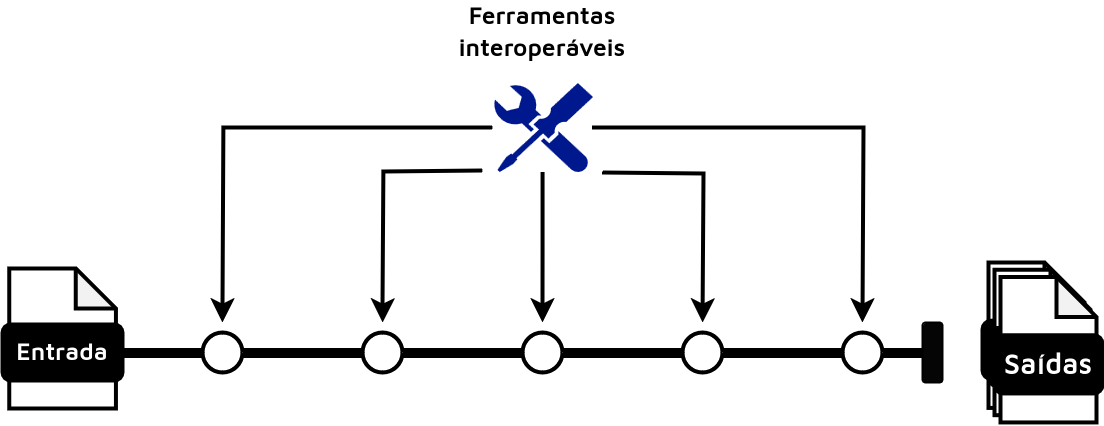
\includegraphics[width=0.7\linewidth]{figure/fluxo_de_trabalho} 

}

\caption{Diagrama que ilustra a estrutura geral de um fluxo de trabalho, compondo ferramentas que realizam diferentes etapas da análise}\label{fig:workflow}
\end{figure}
Tipicamente software é tratado como um ponto adjacente à uma análise científica, e não seu principal produto. Parcialmente isto se dá devido ao modelo de desenvolvimento de software científico atualmente vigente, que se dá por meio de projetos de doutorado e mestrado, dificultando, dessa maneira, manutenção a longo prazo \autocite{altschul2013} \autocite{mangul2019a}. Portanto, produzir metodologias que sejam usáveis a longo prazo sem necessitarem de alta manutenção é essencial. Nesse sentido, a utilização de tecnologias que facilitem a instalação de software, como gerenciadores de ambiente, ou tecnologias capazes de encapsular um ambiente computacional, como contêineres, são indispensáveis para a garantia de reprodutibilidade de qualquer método computacional, por garantirem o isolamento das dependências de um \emph{software} indefinidamente \autocite{kadri2022}.

No entanto, garantir a capacidade de instalação do software é um ponto basal para determinar a qualidade de código científico. Outros princípios, aqui denominados como boas práticas de desenvolvimento de software científicos, são igualmente indispensáveis para que uma metodologia seja utilizável a longo prazo, além de capaz de gerar resultados científicos interpretáveis e consistentes. Além da instalabilidade, alguns outros princípios que garantem a qualidade de um software a longo prazo são uma documentação descritiva, com exemplos práticos de utilização, suporte multi-plataforma \autocite{mangul2019} e, para softwares de processamento de dados, relatórios interativos ou logs acessíveis \autocite{perkel2018}. A implementação de tais princípios em um \emph{software} científico não apenas aumenta sua usabilidade, mas também aumenta as citações de seus artigos, aumentando, consequentemente, o alcance dessas metodologias \autocite{mangul2019a}.

\section{O Ecossistema computacional em Metagenômica}\label{o-ecossistema-computacional-em-metagenuxf4mica}

As metodologias de processamento de dados \gls{16S} em grande parte já estão estabelecidas, dada a idade mais avançada da abordagem. Nesse sentido, vemos que o cerne das abordagens trata de atribuir identificadores únicos às sequências 16S obtidas, caracterizando assim táxons distintos. Esses identificadores podem ser atribuídos através de métodos de agrupamento, caracterizando as abordagens baseadas em \gls{OTU}, que agrupam sequências com pelo menos 97\% de identidade em grupos biológicos distintos, ou abordagens baseadas em \gls{ASV}, que, através de modelos estatísticos, tentam definir variações biológicas reais na sequência - contrastadas com variações devido a erros de sequenciamento, e dessa maneira obter uma resolução taxonômica maior comparada às baseadas em \gls{OTU} \autocite{chiarello2022}. Nesse contexto, observamos metodologias que buscam, a partir dos \gls{OTU} ou \gls{ASV} identificados, inferir abundâncias de vias metabólicas específicas, tirando proveito de bancos de dados de informação curada a respeito desses táxons que possua mapeamento das famílias gênicas de seu genoma a funções biológicas \autocite{douglas2020}. Quanto a fluxos de trabalho para processamento de dados \gls{16S}, destaca-se o \emph{nf-core/ampliseq} \autocite{straub2020}, que implementa várias das boas práticas de software citadas anteriormente, como suporte multi-plataforma, documentação descritiva e exemplificada e relatórios automáticos interativos.

Por outro lado, o campo do desenvolvimento de metodologias para dados de \gls{MS} ainda é bastante fértil, com novas técnicas computacionais desenvolvidas rotineiramente \autocite{liu2021}. De forma geral, podemos agrupar as metodologias em duas grandes categorias: Metodologias livres de montagem, isto é, aquelas que se utilizam apenas da informação contidas nas leituras para obter seus resultados, e metodologias baseadas em montagem, que primeiro realizam a montagem de leituras em sequências contíguas (ou \textit{contigs}), que fornecerá então a base para o processamento seguinte \autocite{breitwieser2019}. Apesar da capacidade que métodos baseados em montagem tem de descobrir novos organismos e montar genomas inéditos, métodos livres de montagem apresentam certas vantagens, sobretudo quando consideramos dados com baixa cobertura de sequência, o que pode resultar em montagens pouco precisas \autocite{ayling2020}.

No que se diz respeito a essas metodologias, vemos que as baseadas em montagem são amplas e cobrem os mais diversos aspectos do processamento de dados de \gls{MS}, com exemplos como nf-core/mag \autocite{krakau2022} e metaphor \autocite{salazar2023}. No entanto, quando observamos métodos livres de montagem, vemos um cenário mais escasso, sobretudo quando consideramos apenas fluxos de trabalho, ou \emph{pipelines}, orquestrados por linguagems de gerenciamento de metodologias científicas, como Nextflow \autocite{ditommaso2017} ou Snakemake \autocite{mölder2021}. No contexto de métodos livres de montagem para dados \gls{MS}, vale ressaltar o fluxo de trabalho MEDUSA \autocite{morais2022}, que apresentou boa sensitividade e flexibilidade para análises de classificação taxonômica e anotação funcional.

Nesse sentido, há a necessidade de desenvolver uma metodologia para dados de \gls{MS} que siga boas práticas de desenvolvimento de software científico e que tenha como princípios norteadores a reprodutibilidade, documentação descritiva e prática e interpretabilidade. Este último ponto que se torna especialmente relevante ao considerarmos a complexidade e a alta dimensionalidade desses dados.

\chapter{Objetivos}\label{obj}

\section{Geral}\label{geral}

Obter uma visão geral do ecossistema computacional em metagenômica atual e como ele se associa
com princípios de desenvolvimento de software científico, desenvolvendo então uma metodologia
para dados de \gls{MS} que possibilite uma análisa metagenômica compreensiva, de forma reprodutível e flexível.

\section{Específicos}\label{especuxedficos}
\begin{itemize}
\tightlist
\item
  Avaliar o atual ferramentário computacional para dados de metagenômica e sua adesão a princípios de desenvolvimento de software sustentável.
\item
  Desenvolver uma metodologia robusta, flexível e acessível para análise de dados de \gls{MS}.
\end{itemize}
\chapter*{CAPÍTULO 1}\label{cap1}
\addcontentsline{toc}{chapter}{CAPÍTULO 1}
\begin{center}
\textbf{Artigo: Bridging the Gaps in Meta-Omic Analysis: Workflows and Reproducibility}
\bigskip\newline
Escrito por: João Vitor Ferreira Cavalcante, Iara Dantas de Souza, Diego Arthur de Azevedo Morais e Rodrigo Juliani Siqueira Dalmolin
\bigskip\newline
\textit{Artigo publicado no periódico OMICS: A Journal of Integrative Biology}

\end{center}
\begin{fichacatalografica}
    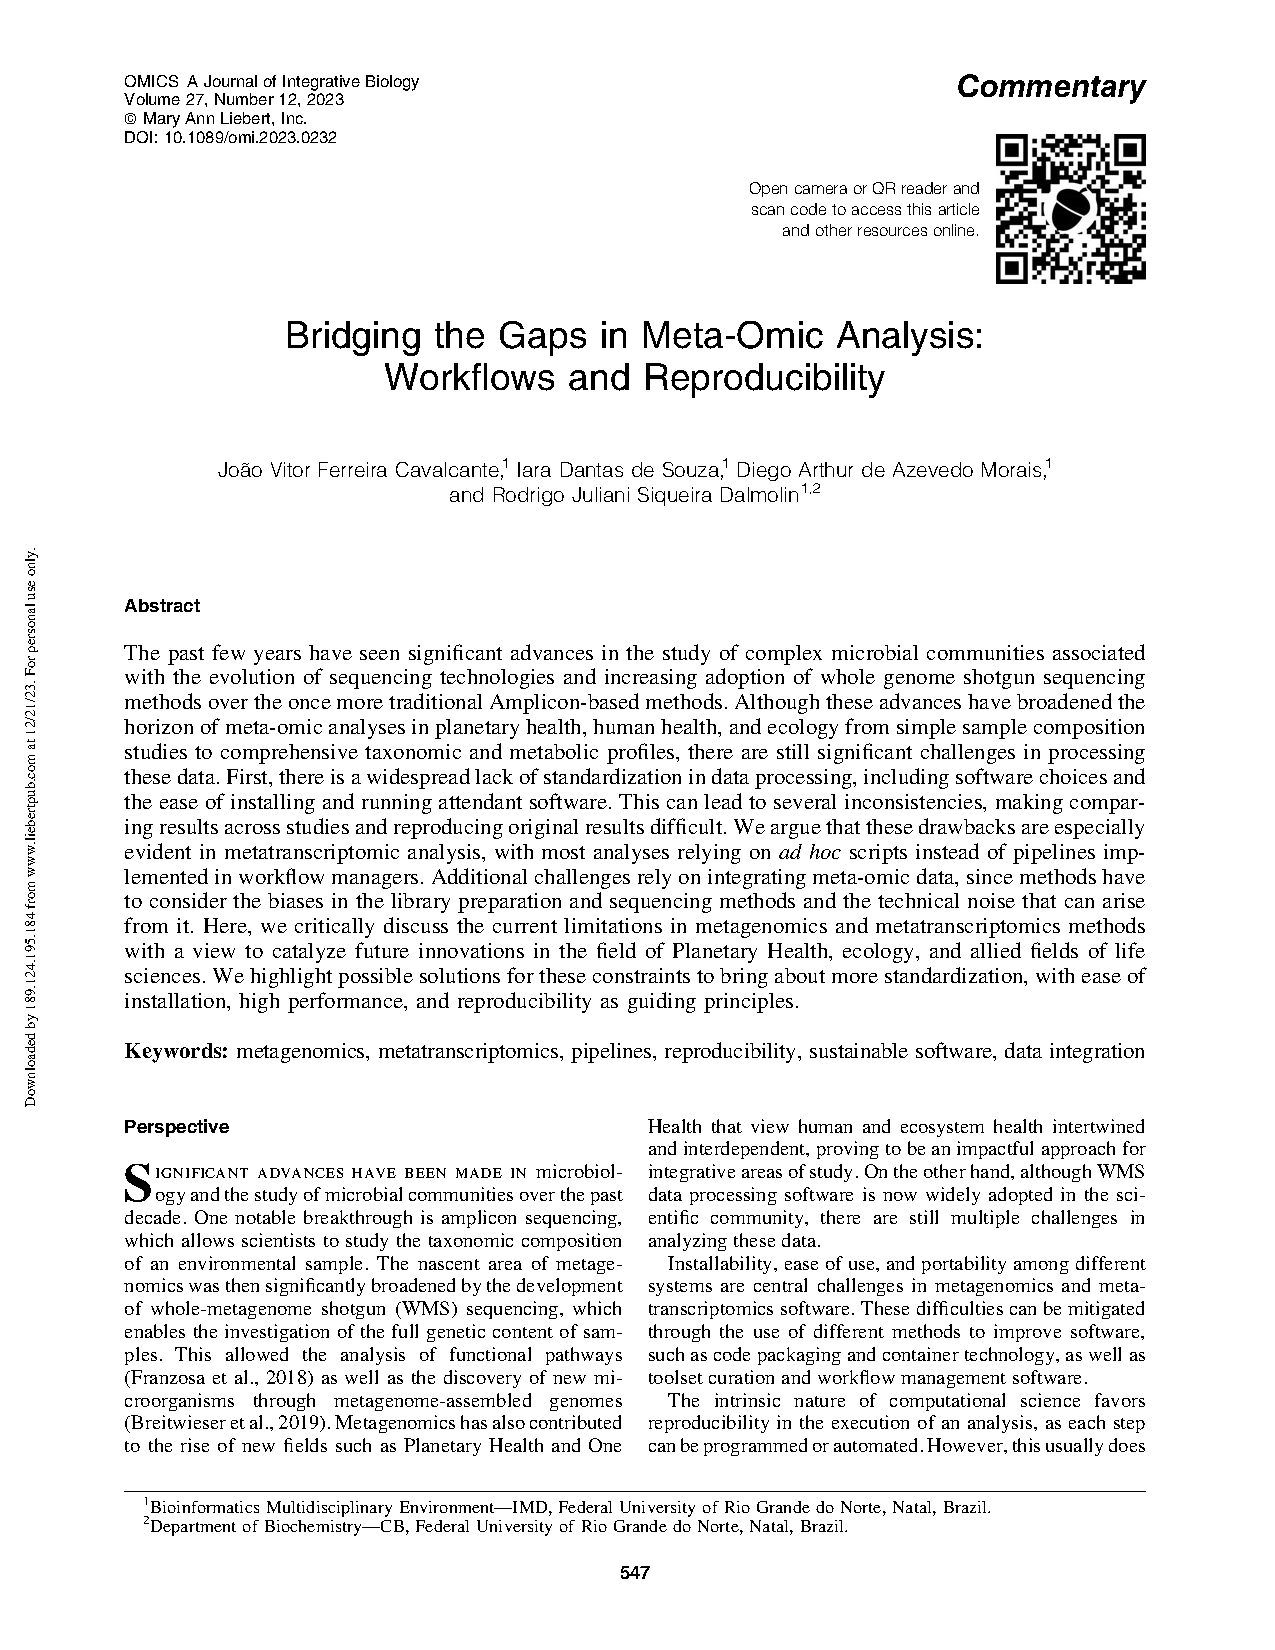
\includepdf[pages={1-}]{papers/paper1.pdf}
\end{fichacatalografica}
\chapter*{CAPÍTULO 2}\label{cap2}
\addcontentsline{toc}{chapter}{CAPÍTULO 2}
\begin{center}
\textbf{Artigo: EURYALE: A versatile Nextflow pipeline for taxonomic classification and functional annotation of metagenomics data}
\bigskip\newline
Escrito por: João Vitor Ferreira Cavalcante, Iara Dantas de Souza, Diego Arthur de Azevedo Morais e Rodrigo Juliani Siqueira Dalmolin
\bigskip\newline
\textit{Artigo submetido ao periódico IEEE Access}

\end{center}
\begin{fichacatalografica}
    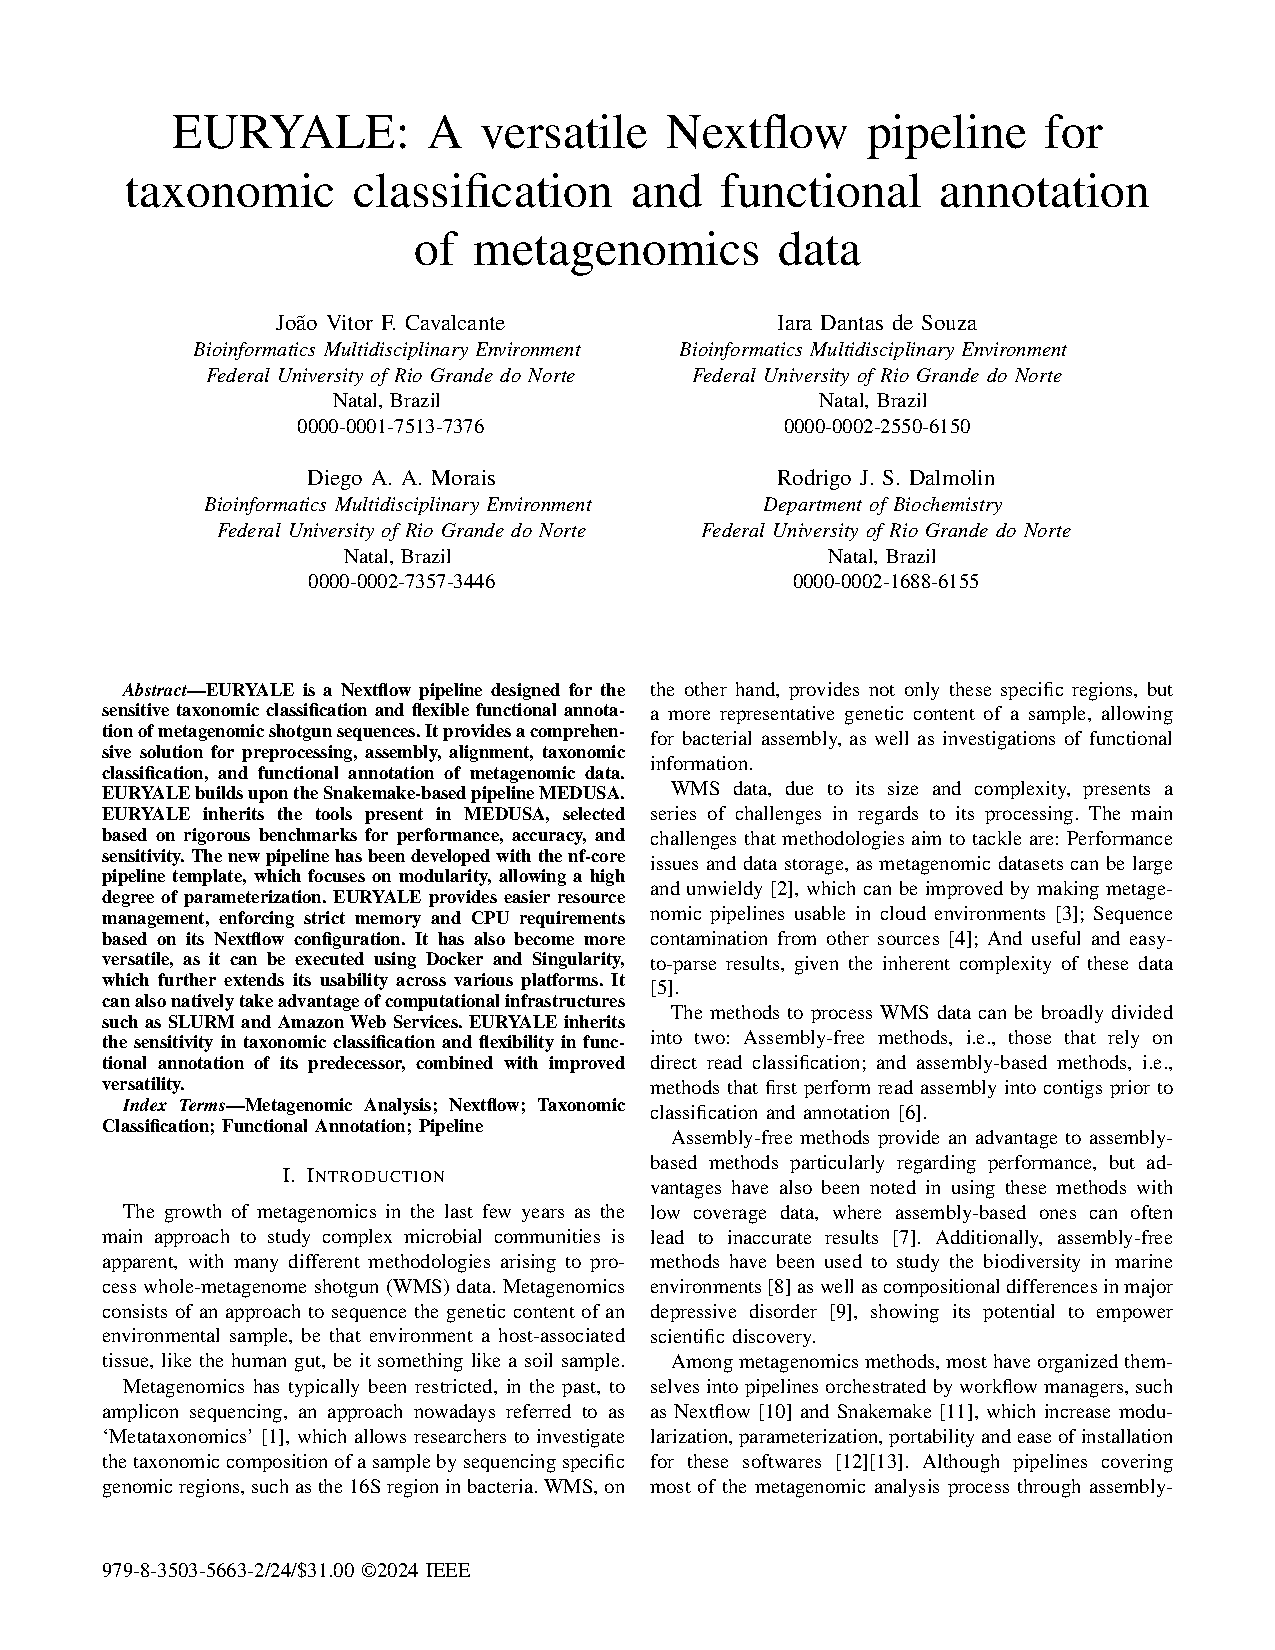
\includepdf[pages={1-}]{papers/paper2.pdf}
\end{fichacatalografica}
\chapter{Discussão}\label{discussuxe3o}

Ao averiguarmos o estado da arte dos fluxos de trabalho computacional presentes na área da metagenômica, pudemos concluir que a adoção de tecnologias de conteinerização e orquestradores de execução ainda é um tanto limitada. Essas limitações tornam-se mais evidentes sobretudo no contexto de metodologias de metagenômica livres de montagem. Tais metodologias são mais escassas e menos computacionalmente intensas quando comparadas às abordagens baseadas em montagem. Ainda assim, elas necessitam processamento adequado, de forma reprodutível, replicável e automatizável, especialmente por possibilitarem uma análise realizável em infraestruturas de menor porte e por possuírem melhor sensibilidade ao tratar dados com baixa cobertura \autocite{ayling2020}, ambos fatores comuns quando se tratando da produção e processamento de dados metagenômicos em ambientes com financiamento científico limitado, como no sul global.

No contexto de possíveis metodologias, decidimos então aplicar os princípios postos para a metodologia MEDUSA \autocite{morais2022}, que apresentou resultados superiores a fluxos de trabalho semelhantes, além de ter obtido suas ferramentas a partir de curadoria manual, com rigorosos processos de benchmarking. Portanto, tomando vantagem da curadoria precedente, decidimos então re-implementar o MEDUSA, utilizando-se agora do gerenciador de pipelines Nextflow a de tecnologias de contêinerização Docker e Singularity.

Nextflow foi escolhido sobretudo devido à facilidade e rapidez de desenvolvimento, conjunta ao suporte multiplataforma mais abrangente que o orquestrador anteriormente escolhido para o MEDUSA, Snakemake. Ademais, Nextflow já foi selecionado como a melhor opção para desenvolvimento de fluxos de trabalho em comparações anteriores \autocite{jackson2021} \autocite{celebi2023}. Outro aspecto que levou à decisão por Nextflow foi a existência da comunidade nf-core, que realiza trabalhos de curadoria de fluxos de trabalho em bioinformática e fornecem templates para a criação de pipelines modulares, altamente parametrizáveis e que possibilitem melhor manutenção a longo prazo \autocite{ewels2020}.

Apesar de reimplementarmos o MEDUSA por completo como EURYALE, também avançamos em algumas limitações do software original, sobretudo interpretabilidade dos dados e parametrização.

Quanto ao primeiro ponto, notávamos uma clara ausência, no MEDUSA, de visualizações e relatórios que forneçam informações preliminares e análises exploratórias acerca do conjunto de dados processado. No entanto, acessibilidade de dados através de relatórios e figuras interativas é essencial para tornar análises mais compreensíveis e reprodutíveis, sobretudo em um campo com complexidade alta de informação, com muitos arquivos gerados por análise, como a metagenômica.

Nesse sentido, primeiro interligamos as diversas ferramentas agora presentes no EURYALE através do MultiQC, um agregador de informação de dados de bioinformática \autocite{ewels2016} que permitiu disponibilizar um relatório interativo e configurável com informações a respeito das etapas de controle de qualidade, classificação taxonômica e do alinhamento que precede a anotação funcional (Figura \ref{fig:multiqc}).
\begin{figure}[H]

{\centering 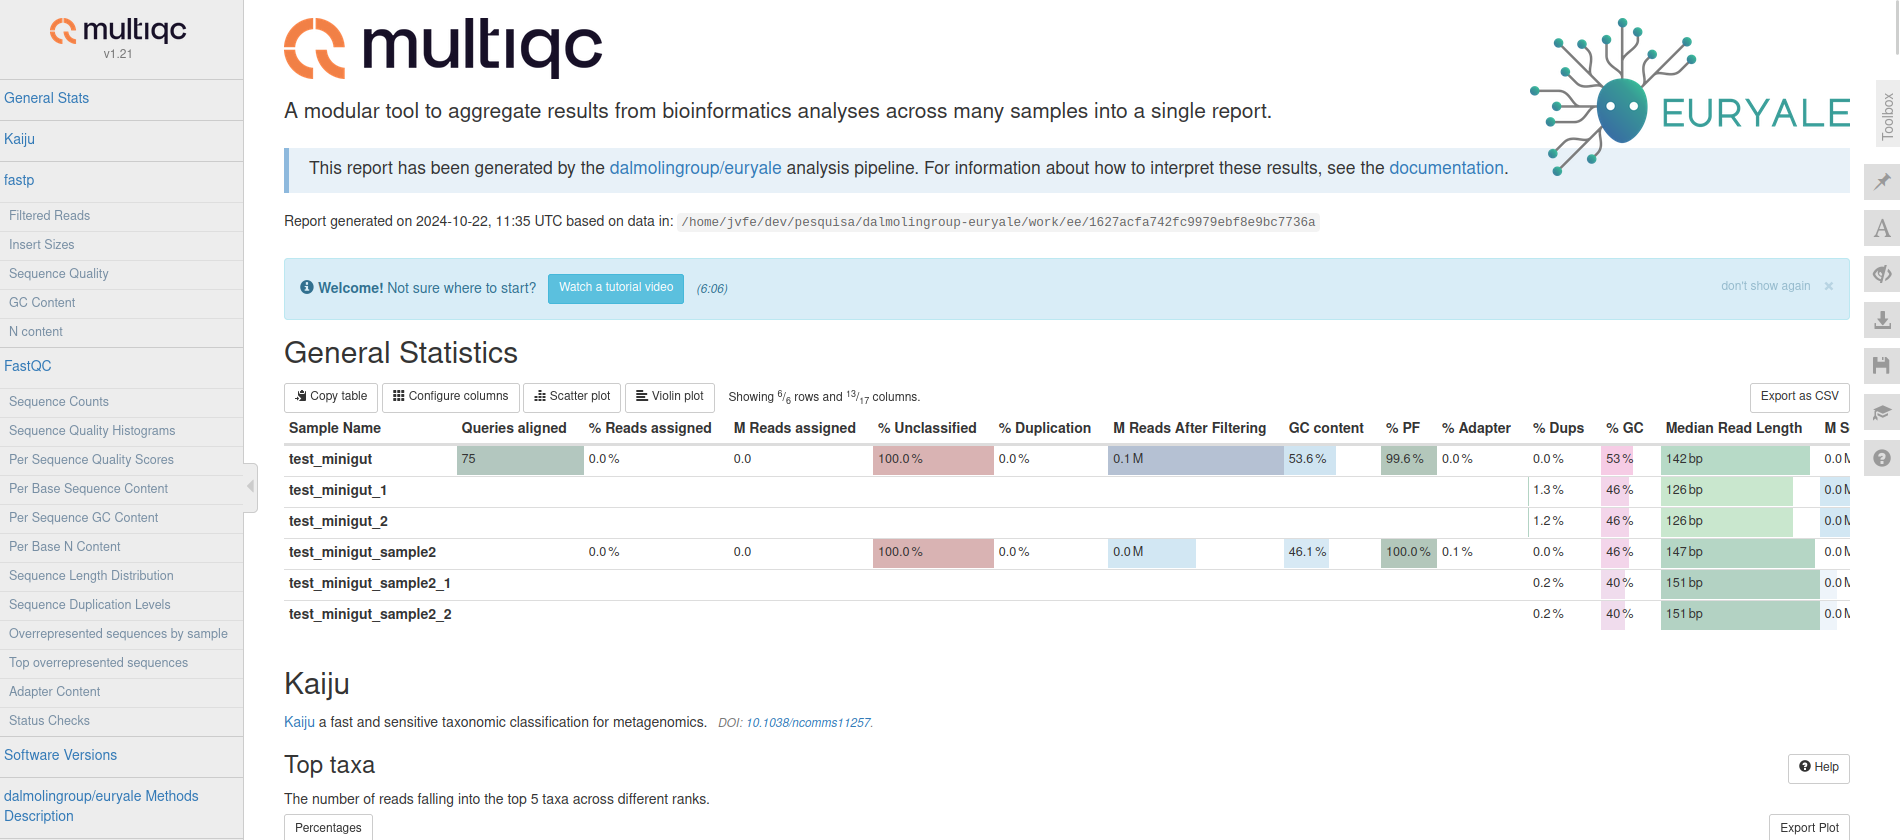
\includegraphics[width=0.7\linewidth]{figure/multiqc_example} 

}

\caption{Exemplo do cabeçalho de um relatório gerado através da ferramenta MultiQC, implementada como parte integrante do EURYALE.}\label{fig:multiqc}
\end{figure}
Ademais, através da implementação de uma nova ferramenta, MicroView, também inclusa no EURYALE, disponibilizamos também ao usuário métricas pré-calculadas de diversidade, ilustrando, de forma inicial e exploratória, o quadro geral resultante da classificação taxonômica (Figura \ref{fig:microview}).
\begin{figure}[H]

{\centering 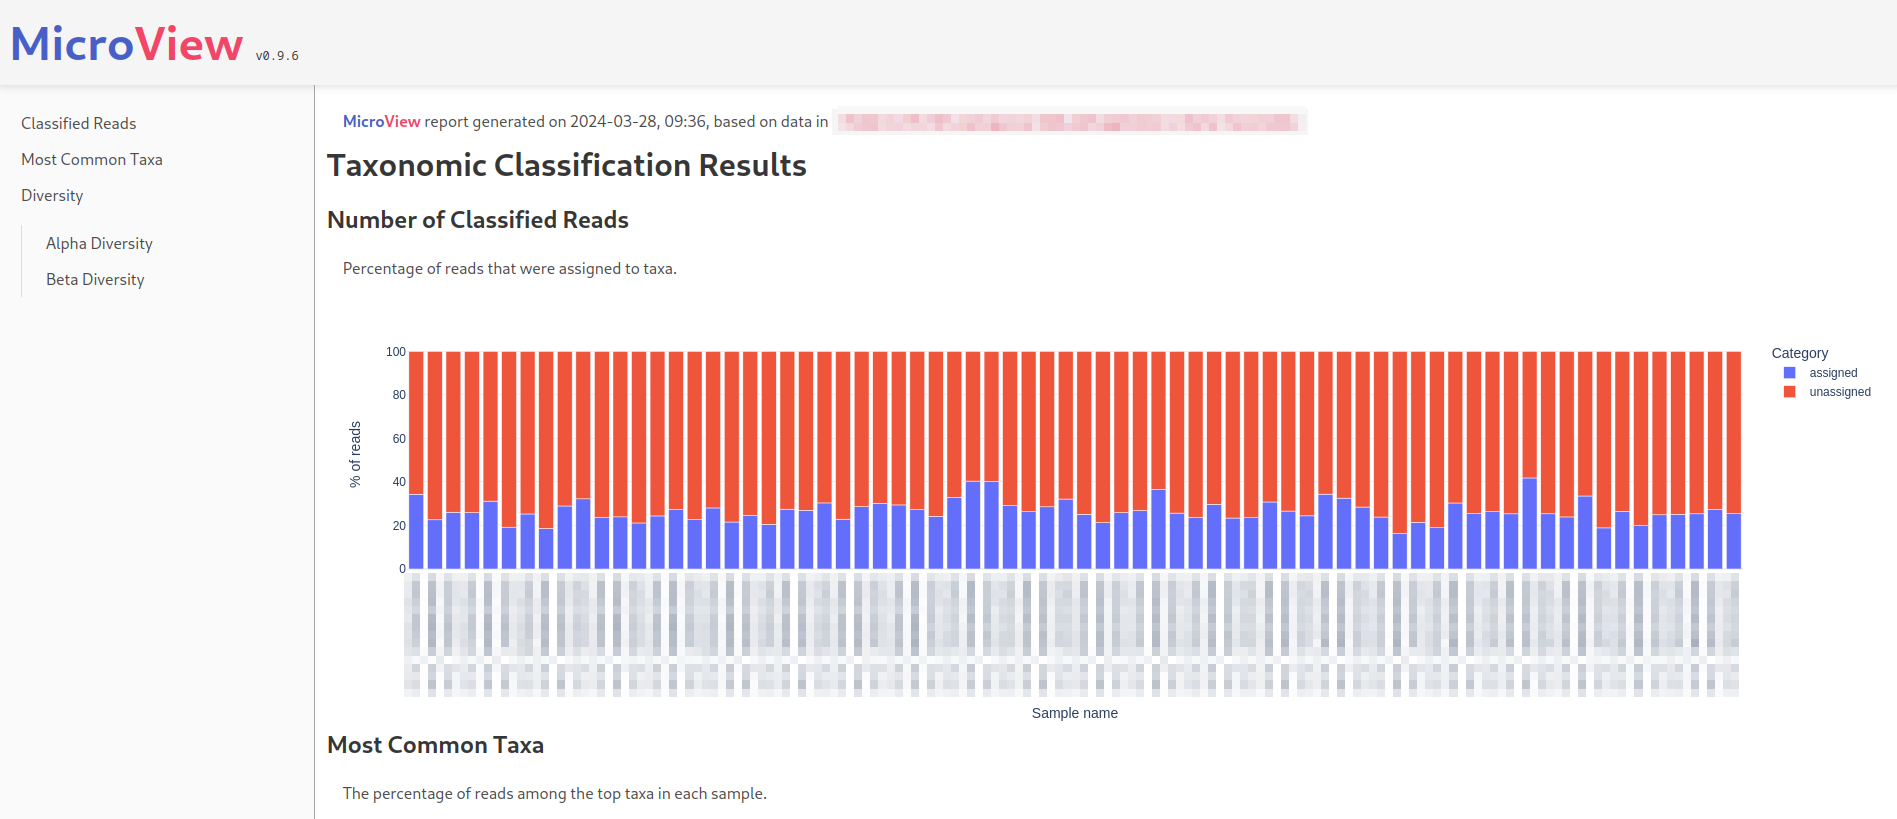
\includegraphics[width=0.7\linewidth]{figure/microview_example} 

}

\caption{Exemplo do cabeçalho de um relatório gerado através da ferramenta Microview, escrita em Python e implementada como parte integrante do EURYALE.}\label{fig:microview}
\end{figure}
O MicroView também atua como um pacote na linguagem Python de programação, possibilitando sua execução fora do fluxo de trabalho. De forma geral, tais relatórios, com visualizações interativas, aumentam a acessibilidade de dados das análises realizadas com o EURYALE, facilitando não apenas a exploração inicial e a geração de descobertas científicas pelos pesquisadores usuários da metodologia, mas também a exploração posterior dos resultados, promovendo re-análises \autocite{perkel2018}.

Vale ressaltar também os aprimoramentos em padronização de software e parametrização trazidos da mudança do MEDUSA para o EURYALE. Ao implementarmos a metodologia, optamos por utilizar a infraestrutura da nf-core, uma comunidade que busca padronizar o desenvolvimento de fluxos de trabalho que utilizam Nextflow, com ênfase em modularidade, testes contínuos e documentação \autocite{ewels2020}. A comunidade implementa uma suíte de software em Python para a criação e manutenção de fluxos de trabalho (\url{https://nf-co.re/docs/nf-core-tools/installation}), que foi amplamente utilizada no desenvolvimento do EURYALE. Ao utilizarmos das ferramentas e diretrizes da nf-core, pudemos superar algo que foi a principal crítica de usuários em relação ao MEDUSA: A estaticidade das referências e a pouca parametrização.

Quanto ao primeiro ponto, optamos por uma solução que possibilite a utilização de bancos de dados referência equivalentes aos utilizados pelo MEDUSA, que é o que tomamos como padrão da análise. Nesse sentido, implementamos uma entrada alternativa ao fluxo de trabalho (\texttt{-entry\ download}`), que possibilita que os usuários transfiram os bancos de dados referência para sua máquina de análise, alimentando assim o \emph{pipeline} propriamente dito (Figura \ref{fig:entries}).
\begin{figure}[H]

{\centering 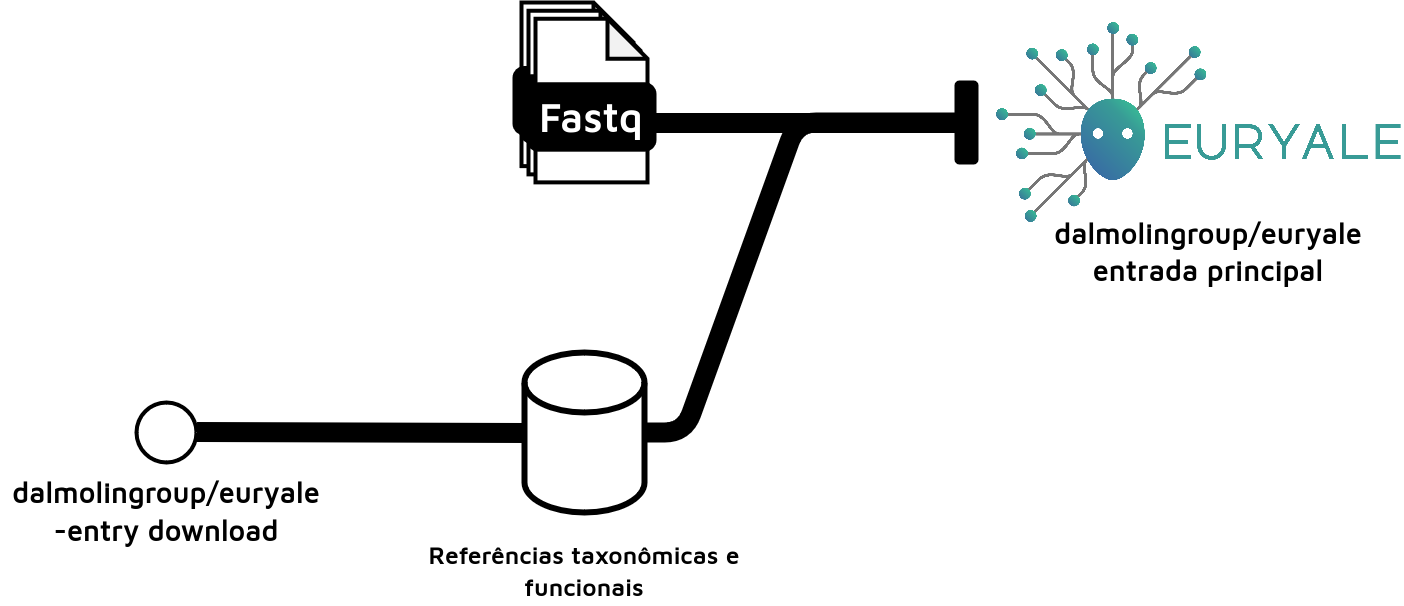
\includegraphics[width=0.7\linewidth]{figure/euryale_entries.drawio} 

}

\caption{Diagrama ilustrando como a entrada de download do EURYALE adquire os bancos de dados que alimentam a entrada principal. Com uma análise típica do zero sendo constituída por ambas etapas.}\label{fig:entries}
\end{figure}
Apesar disso, devido à modularidade advinda do \emph{template} \emph{nf-core}, o EURYALE é modelado para funcionar com quaisquer outro banco de dado compatível com as suas ferramentas integrantes. Dessa maneira, o usuário pode tanto modificar os parâmetros de \emph{download} na entrada específica, quanto modificar diretamente os parâmetros de referência presentes na entrada principal do \emph{pipeline}, caso ele possua referências pré-adquiridas. Esses detalhes funcionais distinguem a usabilidade do EURYALE com a de seu precedente, não requerendo que os usuários alterem o código fonte para utilizar referências diferentes.

Além disso, adicionamos mais parâmetros ao EURYALE, parâmetros estes tanto que alterem as etapas de análise quanto aqueles que alteram os recursos computacionais alocados a estas etapas. A exemplo dessa mudança, podemos ver como a metodologia agora apoia um passo opcional de montagem, semelhante ao descrito no artigo original do MEDUSA, no entanto não aplicado diretamente na sua versão orquestrável original. O novo fluxo de trabalho também oferece mais opções de classificação taxonômica, além de parâmetros que possibilitam desabilitar diferentes passos de análise, como a descontaminação de leituras do hospedeiro, possibilitando que a abordagem se adapte a diferentes contextos de análise. Adicionalmente, outro ponto originado pela utilização do template \emph{nf-core} são os diferentes rótulos de alocação de recursos, que permitem um gerenciamento fácil, da quantidade de recursos que pode ser alocada a cada passo de análise, através de um único arquivo de configuração. Essa adição permite que a metodologia seja executada em diferentes infraestruturas computacionais.

Em última instância, vale ressaltar como a utilização do \emph{template} \emph{nf-core} também possibilita a implantação do fluxo de trabalho na \emph{Seqera Platform}, com a geração automática de uma interface gráfica, permitindo a usuários executar a metodologia sem necessariamente utilizarem uma interface em linha de comando, dado que, é claro, possuam cadastro na plataforma (Figura \ref{fig:seqeraplat}).
\begin{figure}[H]

{\centering 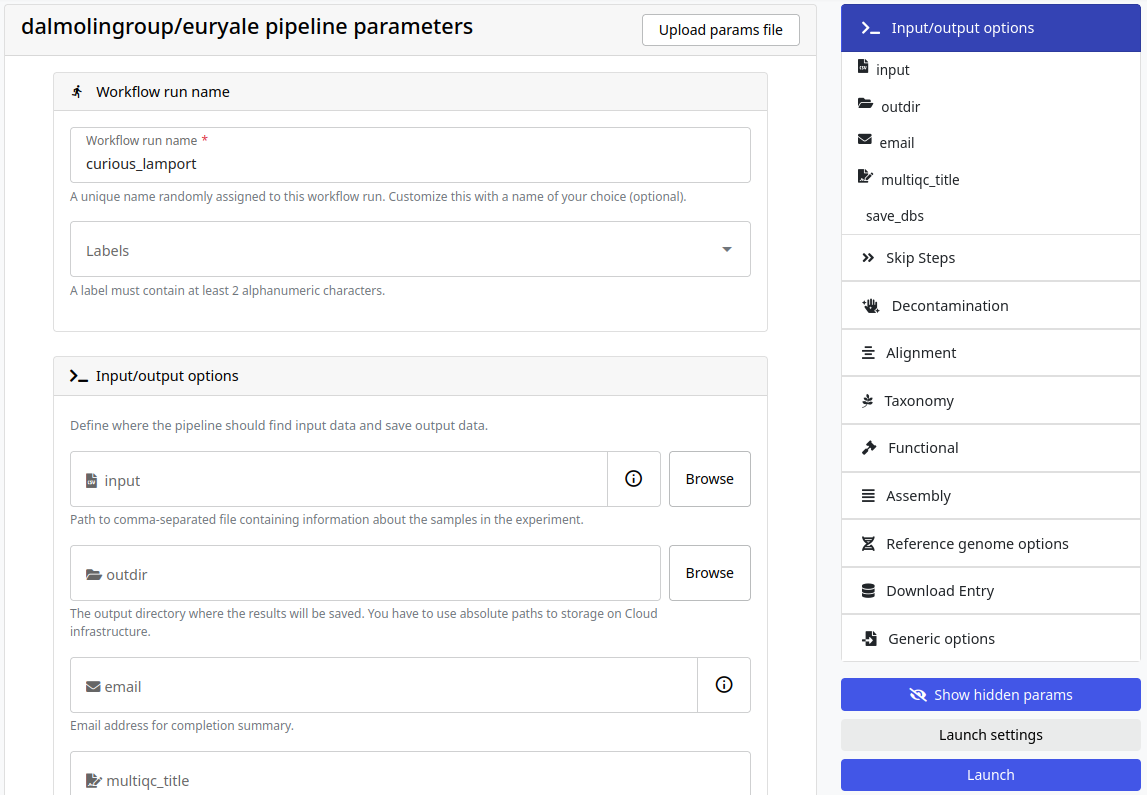
\includegraphics[width=0.7\linewidth]{figure/seqera_platform_example} 

}

\caption{Porção inicial da interface gráfica do EURYALE na Seqera Platform (<https://cloud.seqera.io/>). Através desse formulário usuários podem selecionar os parâmetros a serem utilizados para a execução do fluxo de trabalho.}\label{fig:seqeraplat}
\end{figure}
\chapter{Conclusão}\label{conclusuxe3o}

Ao averiguar o estado do desenvolvimento de \emph{software} em meta-ômica, pudemos observar
uma baixa aderência a boas práticas de desenvolvimento, sobretudo no que tange \emph{pipelines}
de análise de dados. Nesse sentido, nos baseamos em uma metodologia anterior parar desenvolvermos um fluxo de trabalho, denominado EURYALE,
que possibilita uma análise completa de dados de \gls{MS}, e possui isolamento de dependências, alta parametrização, relatórios automáticos com visualizações interativas e uma documentação expansiva, com exemplos práticos.
Nossa iniciativa com o desenvolvimento do EURYALE não só avança ideais de desenvolvimento de \emph{software} científico, como também facilita com que haja um processamento de dados acurado, estável e sensível.
No entanto, deve-se ressaltar que, apesar de avançarmos na abordagem fundamental da metagenômica, metodologias de integração de dados
meta-ômicos, isto é, metagenômico e metatranscriptômico, ainda são relativamente escassas. Este aspecto se torna ainda mais evidente ao considerarmos fluxos de trabalho automatizados que sigam boas práticas de desenvolvimento de \emph{software}.
Portanto, futuras iniciativas devem ser orientadas para que a realização desses futuros métodos siga também os princípios delineados no presente trabalho.

\postextual

\begingroup

\printbibliography[title=REFERÊNCIAS]

\endgroup

\markboth{Referências}{REFERÊNCIAS}

\chapter{ANEXO I}\label{anexo-i}
\begin{center}
Segue abaixo a documentação servida no \textit{site} do EURYALE
\bigskip\newline
\textit{Acessada na data \today}
\end{center}
\begin{fichacatalografica}
    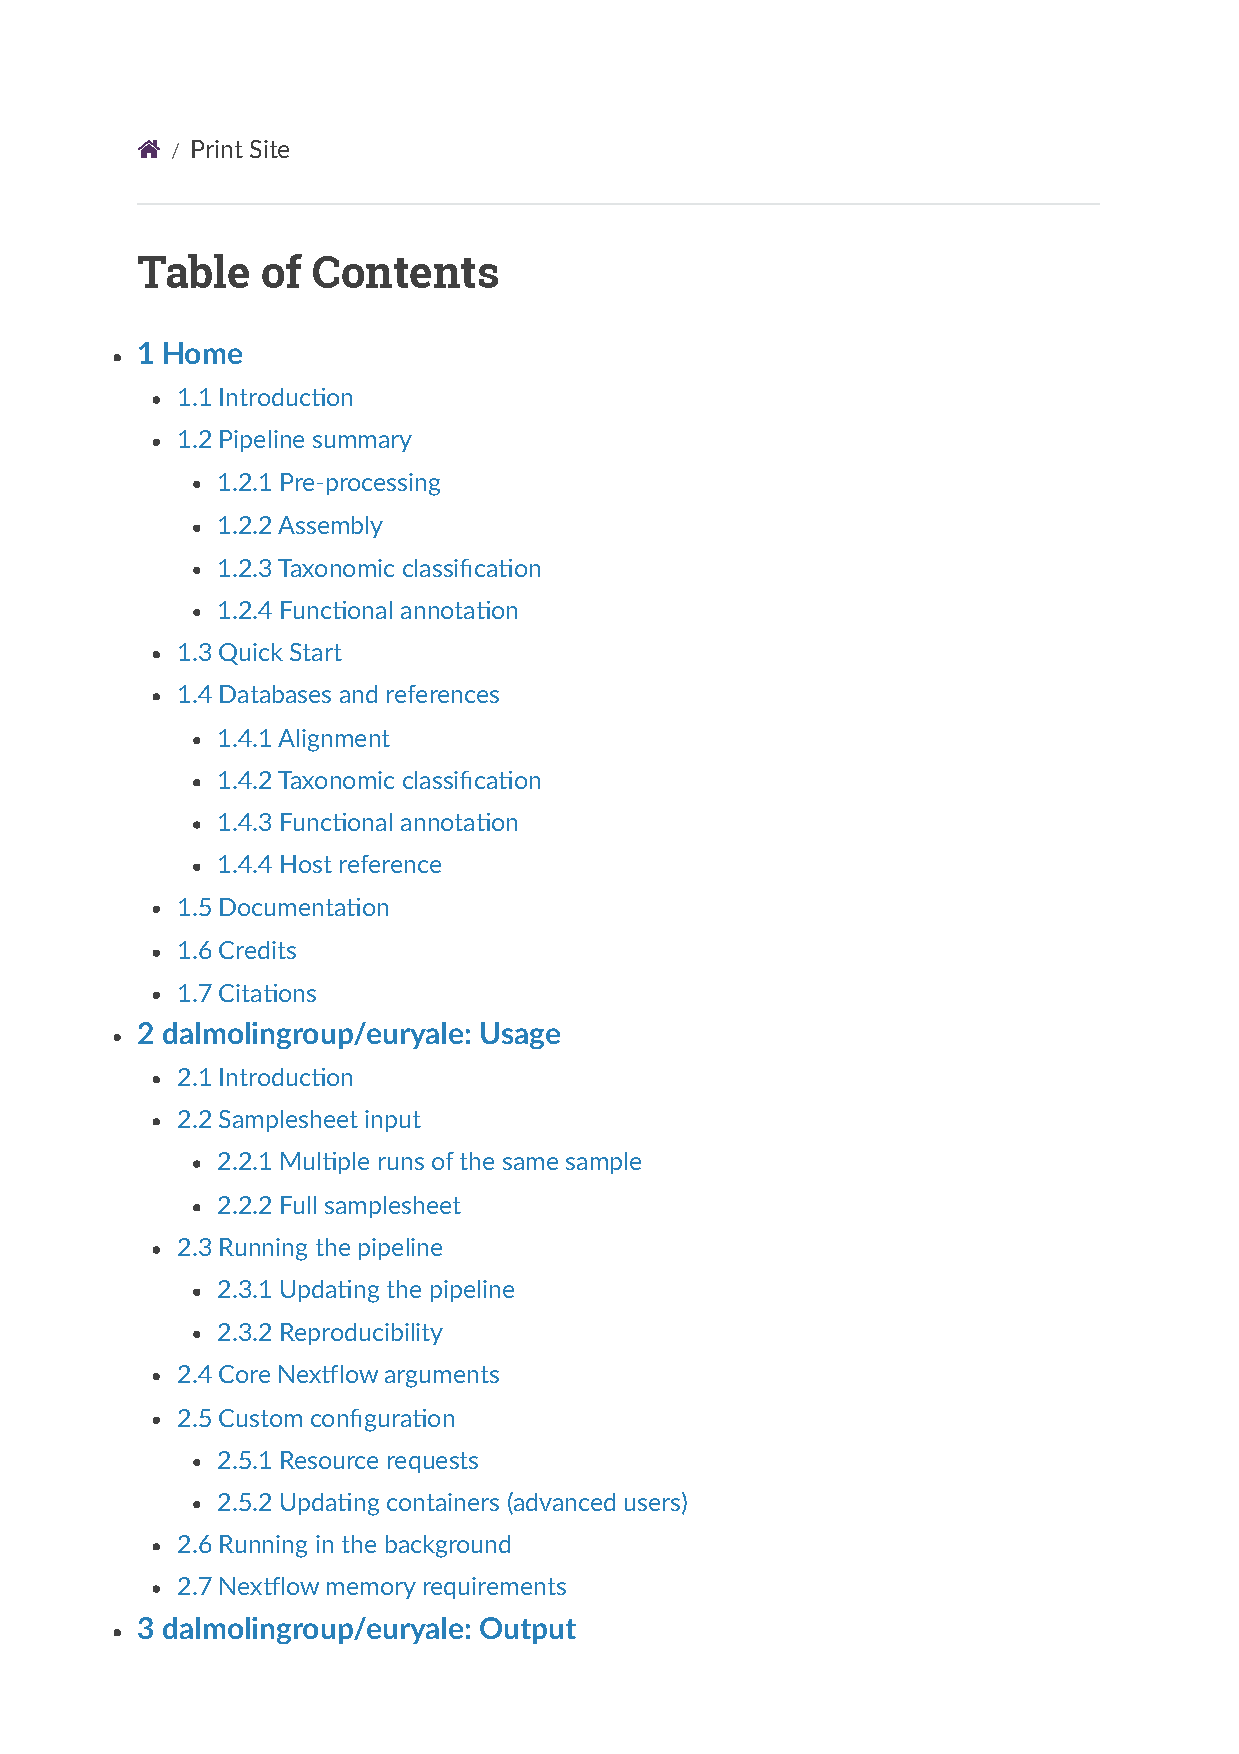
\includepdf[pages={1-}]{papers/documentation.pdf}
\end{fichacatalografica}
% ----------------------------------------------------------
% Glossário
% ----------------------------------------------------------
%
% Consulte o manual da classe abntex2 para orientações sobre o glossário.
%
%\glossary

%---------------------------------------------------------------------
% INDICE REMISSIVO
%---------------------------------------------------------------------
%\phantompart
%\printindex
%---------------------------------------------------------------------

\end{document}
